\documentclass[12pt,t]{beamer}
\usepackage{graphicx}
\usepackage[vlined]{algorithm2e}
\usepackage{times}
\usepackage{calc}
\usepackage{url}
\usepackage{soul}
\usepackage{graphicx}
\usepackage{multirow, hhline}
\usepackage{array, booktabs}
\usepackage{amsmath}
\usepackage{amssymb}
\usepackage{relsize}
\usepackage{multirow}
\usepackage{booktabs}
\usepackage{pagecolor}
\usepackage{lipsum}
\usepackage{capt-of}
\usepackage{booktabs}

\usepackage{graphicx}
\usepackage{multicol}
\usepackage[T1]{fontenc}
\usepackage{ae}
\graphicspath{{fig/}}
\setbeameroption{hide notes}
\setbeamertemplate{note page}[plain]

\usetheme{default}
\beamertemplatenavigationsymbolsempty
\hypersetup{pdfpagemode=UseNone}

\usefonttheme{professionalfonts}
\usefonttheme{serif}
\usepackage{fontspec}
\setmainfont{Karla}
\setbeamerfont{note page}{family*=pplx,size=\footnotesize} % Palatino for notes

\definecolor{foreground}{RGB}{70,70,70}
\definecolor{background}{RGB}{249, 249, 249} %24,24,24
%\definecolor{title}{RGB}{107,174,214} %107,174,214
\definecolor{title}{RGB}{70,70,70}
\definecolor{gray}{RGB}{0,0,0}
\definecolor{subtitle}{RGB}{70,70,70}
\definecolor{hilight}{RGB}{102,255,204}
\definecolor{vhilight}{RGB}{255,111,207}

\setbeamercolor{titlelike}{fg=title}
\setbeamercolor{subtitle}{fg=subtitle}
\setbeamercolor{institute}{fg=gray}
\setbeamercolor{normal text}{fg=foreground,bg=background}


\setbeamercolor{item}{fg=foreground} % color of bullets
\setbeamercolor{subitem}{fg=gray}
\setbeamercolor{itemize/enumerate subbody}{fg=gray}
\setbeamertemplate{itemize subitem}{{\textendash}}
\setbeamerfont{itemize/enumerate subbody}{size=\footnotesize}
\setbeamerfont{itemize/enumerate subitem}{size=\footnotesize}

\setbeamercolor{block title}{fg=white,bg=gray!70}
\setbeamercolor{block body}{fg=black,bg=gray!10}
\setbeamercolor{block title alerted}{fg=red,bg=gray!40}
\setbeamercolor{block title example}{fg=black,bg=green!20}
\setbeamercolor{block body example}{fg=black,bg=green!5}
\setbeamerfont{block title}{series=\bfseries}

\hypersetup{colorlinks,linkcolor=foreground,urlcolor=foreground}


\setbeamertemplate{footline}{%
    \raisebox{5pt}{\makebox[\paperwidth]{\hfill\makebox[20pt]{\color{gray}
          \scriptsize\insertframenumber}}}\hspace*{5pt}}

\addtobeamertemplate{note page}{\setlength{\parskip}{12pt}}


\newcommand{\bi}{\begin{itemize}}
\newcommand{\ei}{\end{itemize}}
\newcommand{\ig}{\includegraphics}
\newcommand{\subt}[1]{{\footnotesize \color{subtitle} {#1}}}

\let\emph\relax % there's no \RedeclareTextFontCommand
\DeclareTextFontCommand{\emph}{\bfseries\em}


\setbeamertemplate{frametitle}
{\vskip4pt
  \leavevmode
%\hbox{%
\begin{beamercolorbox}[wd=\paperwidth,ht=2ex,dp=0ex]{frametitle}%
\underline{\makebox[\paperwidth][l]{\hspace*{10pt}
\large {{\insertframetitle}}}}
\end{beamercolorbox}
%  }%
}

%\setbeamercolor{frametitle}{fg=yellow,bg=red}

\begin{document}

\AtBeginSection[]{
  \begin{frame}
  \vfill
  \centering
  \begin{beamercolorbox}[sep=8pt,center,shadow=true,rounded=true]{title}
    \underline{\makebox[0.6\paperwidth][l]{
\large {{\insertsectionhead}}}}
  \end{beamercolorbox}
  \vfill
  \end{frame}
}

\title{\large{Lecture \#0: Introduction to CS109A}}
\subtitle{CS 109A, STAT 121A, AC 209A: Data Science}
\author{Pavlos Protopapas \and Kevin Rader}
%\institute{Harvard University}
\date{}
\titlegraphic{
   
\includegraphics[height=2cm]{iacs}
\includegraphics[height=2cm]{hogwarts}
}
{
\setbeamertemplate{footline}{} % no page number here
\frame{
  \titlepage
  
}
}


\begin{frame}{Lecture Outline}
\tableofcontents
\end{frame}

%%%%%%%%%%%%%%%%%%%%%%%%%%%%%%%%%%%%%%%%%%%%%%%%%%%%%%%%%%%%%%%%%%%%%%%%%%%%%%
\section{What is Data Science}

%%%%%%%%%%%%%%
\begin{frame}{Slide Title} 

\end{frame}

%%%%%%%%%%%%%%%%%%%%%%%%%%%%%%%%%%%%%%%%%%%%%%%%%%%%%%%%%%%%%%%%%%%%%%%%%%%%%%
\section{What is This Class?}

%%%%%%%%%%%%%%
\begin{frame}{Slide Title} 

\end{frame}

%%%%%%%%%%%%%%%%%%%%%%%%%%%%%%%%%%%%%%%%%%%%%%%%%%%%%%%%%%%%%%%%%%%%%%%%%%%%%%
\section{Practicing Data Science}

%%%%%%%%%%%%%%
\begin{frame}{The Data Science Process} 
The Data Science Process is similar to the scientific process - one of observation, model building, analysis and conclusion:
\vskip0.2cm
\begin{itemize}
\item  Ask questions
\item  Data Collection
\item  Data Exploration
\item  Data Modeling
\item  Data Analysis
\item  Visualization and Presentation of Results 
\end{itemize}
\vskip0.2cm
\textbf{Note:} This process is by no means linear!
\end{frame}

%%%%%%%%%%%%%%
\begin{frame}{Analyzing Hubway Data} 
\vskip-0.2cm
\textbf{Introduction: } Hubway is metro-Boston's public bike share program, with more than 1600 bikes at 160+ stations across the Greater Boston area. Hubway is owned by four municipalities in the area.
\vskip0.2cm
By 2016, Hubway operated 185 stations and 1750 bicycles, with 5 million ride since launching in 2011. 
\vskip0.4cm
\textbf{The Data: } In April 2017, Hubway held a Data Visualization Challenge at the Microsoft NERD Center in Cambridge, releasing 5 years of trip data.
\vskip0.4cm
\textbf{The Question: } What does the data tell us about the ride share program?
\end{frame}

%%%%%%%%%%%%%%
\begin{frame}{The Data Exploration/Question Refinement Cycle} 
\only<1>{
\vskip-0.4cm
Our original question:
\begin{center}
\emph{`What does the data tell us about the ride share program?'}
\end{center} 
is a reasonable slogan to promote a hackathon. It is not good for guiding scientific investigation.
\vskip0.2cm
Before we can refine the question, we have to look at the data!
\begin{center}
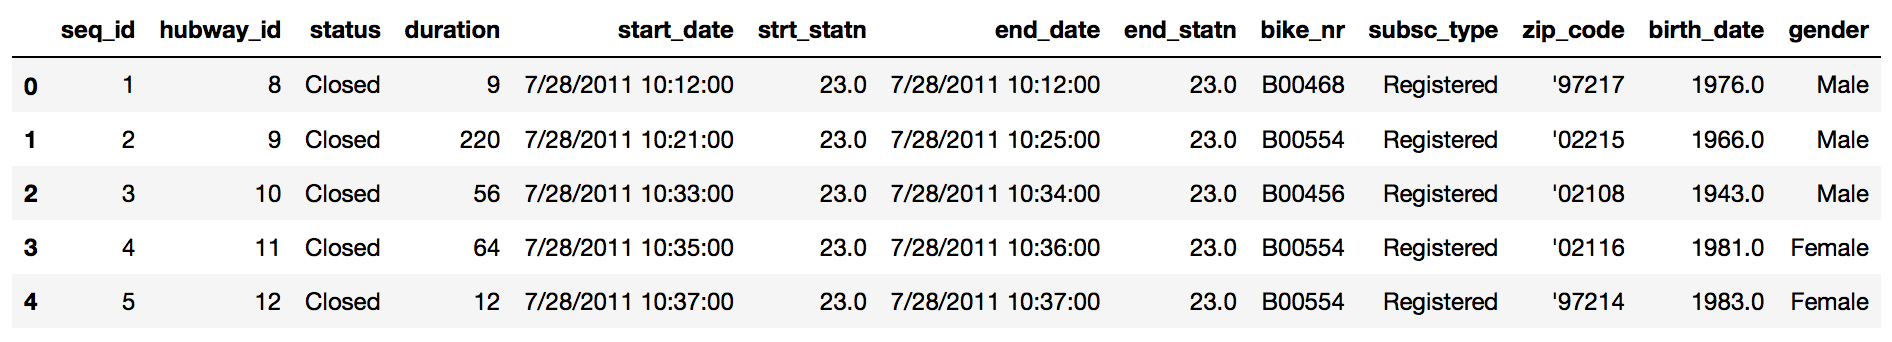
\includegraphics[width=108mm]{Lecture0_g1}
\end{center}
Based on the data, what kind of questions can we ask?
}
\only<2->{
\begin{itemize}
\only<2-5>{
\item \textbf{Who?} Who's using the bikes?
\vskip0.2cm
Refine into specific hypotheses:
\vskip0.2cm
\begin{itemize}
\item<3-> More men or more women?
\vskip0.2cm
\item<4-> Older or younger people?
\vskip0.2cm
\item<5-> Subscribers or one time users?
\end{itemize}
}
\only<6-9>{
\item \textbf{Where?} Where are bikes being checked out?
\vskip0.2cm
Refine into specific hypotheses:
\vskip0.2cm
\begin{itemize}
\item<7-> More in Boston than Cambridge?
\vskip0.2cm
\item<8-> More in commercial or residential?
\vskip0.2cm
\item<9-> More around tourist attractions?
\end{itemize}
\vskip0.2cm
\only<9>{\emph{Sometimes the data is given to you in pieces and must be merged!}}
}
\only<10-13>{
\item \textbf{When?} When are the bikes being checked out?
\vskip0.2cm
Refine into specific hypotheses:
\vskip0.2cm
\begin{itemize}
\item<11-> More during the weekend than on the weekdays?
\vskip0.2cm
\item<12-> More during rush hour?
\vskip0.2cm
\item<13-> More during the summer than the fall?
\end{itemize}
\vskip0.2cm
\only<13>{\emph{Sometimes the feature you want to explore doesn't exist in the data, and must be engineered!}}
}
\only<14>{
\item \textbf{Why?} For what reasons/activities are people checking out bikes?
\vskip0.2cm
Refine into specific hypotheses:
\vskip0.2cm
\begin{itemize}
\item More bikes are used for recreation than commute?
\vskip0.2cm
\item More bikes are used for touristic purposes?
\vskip0.2cm
\item Bikes are use to bypass traffic?
\end{itemize}
\vskip0.2cm
\emph{Do we have the data to answer these questions with reasonable certainty?} 
\vskip0.2cm
\emph{What data do we need to collect in order to answer these questions?}
\vskip0.2cm
}

\only<15>{
\item \textbf{How?} Questions that combine variables.
\vskip0.2cm
\begin{itemize}
\item How does user demographics impact the duration the bikes are being used? Or where they are being checked out?
\vskip0.2cm
\item How does weather or traffic conditions impact bike usage?
\vskip0.2cm
\item How do the characteristics of the station location affect the number of bikes being checked out?
\end{itemize}
\vskip0.2cm
How questions are about modeling relationships between different variables.
}
\end{itemize}
}
\end{frame}

\begin{frame}{Inspirations for Data Viz/Exploration}
\vskip-0.4cm 
So how well did we do in formulating creative hypotheses and manipulating the data for answers?
\vskip0.2cm
Check out the winners of the Hubway Challenge:
\vskip0.2cm
\begin{center}
\emph{http://hubwaydatachallenge.org}\\
\vskip0.2cm
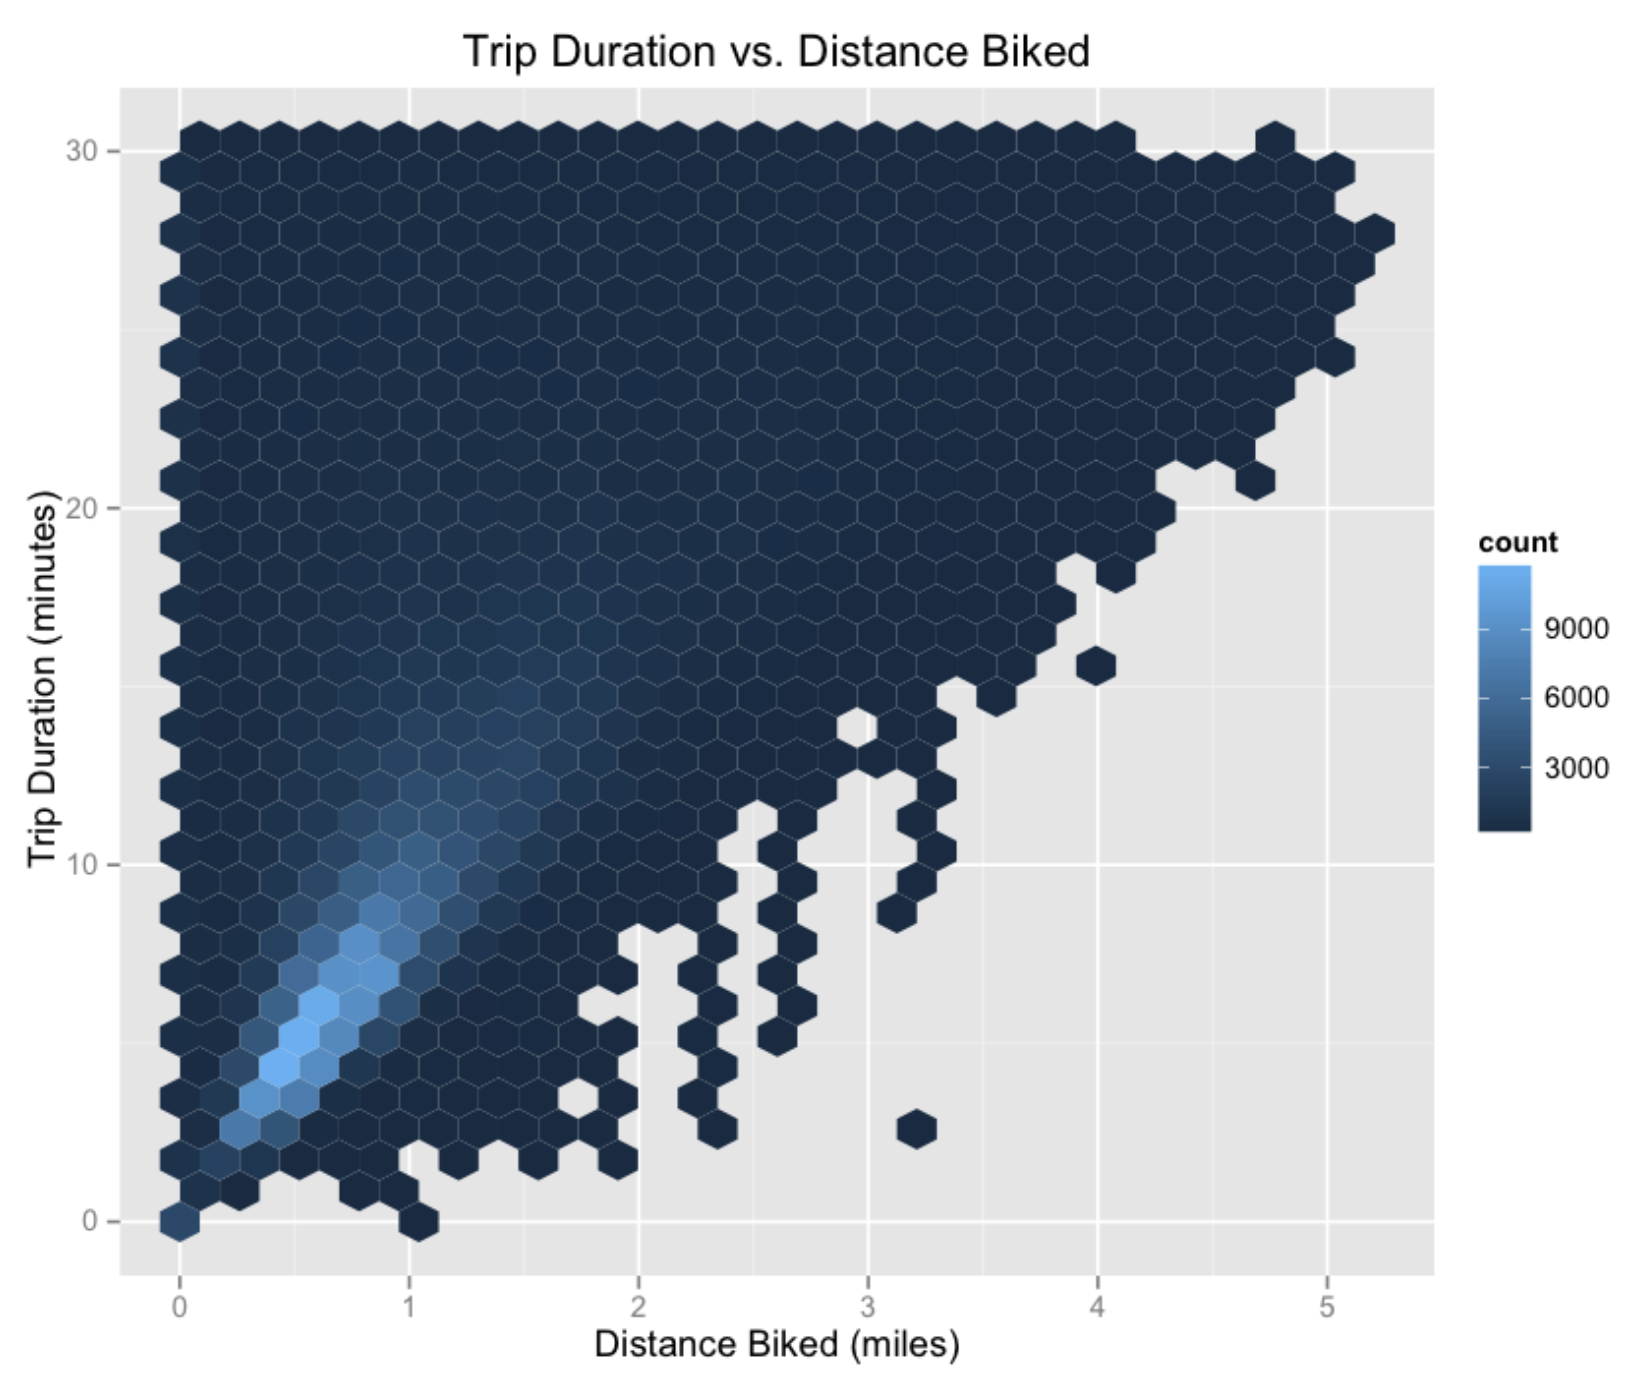
\includegraphics[width=60mm]{Lecture0_g3}
\end{center}
\end{frame}

\end{document}
